% -----------------------------*- LaTeX -*------------------------------
\documentclass[11pt]{report}
\usepackage{epstopdf}
\usepackage{hw_style}
\usepackage{graphicx}
\usepackage{dsfont}
\usepackage{caption}
\usepackage{subcaption}


\def\exp#1{\mathop{\mathrm{exp}}\left( #1\right)}
\usepackage{amsmath}
\begin{document}
\scribe{Ankush Gupta} % required
\hwnumber{1} % required, must be a number
\duedate{Feb 25} % required, omit year
\maketitle
% ----------------------------------------------------------------------

\section*{$\text{CO}_2$ Level Forecasting}
I followed two approaches for forecasting this time series --- (1) decomposing the series into long-term and short-term trends (2) using gaussian process regression.

\subsection*{Series Decomposition}
Clearly, there are (at least) two trends in the given time series --- (1) $f_L(t)$ Long term increase (2) $f_S(t)$ Short term almost sinusoidal trend. Hence, my analysis for this time series was aimed at finding these two components such that $f_{CO_2}(t) \approx f_L(t) + f_S(t)$

\subsubsection*{Fitting Long Term Trend}
Since, many natural phenomena follow the exponential trend because of their dynamics being $\dfrac{dx}{dt}\propto \alpha x$, I first tried fitting an exponential curve $f_L(t) = \beta e^{\alpha t}$, by taking logs and using ordinary least squares. The fit didn't look right \footnote{which was quite surprising for me.}, so I tried decomposing it in terms of the polynomial basis $\{1,x,x^2,x^3,...\}$ using least-squares.\\

To get rid of the sinusoidal trend, I used a low-pass filter to uncover the long-term trend \footnote{Note: I could have used the raw-curve (without any pre-processing/ filtering) to find coefficients of the polynomial basis elements.} (more specifically, I used a Butterworth filter with the cut-off frequency determined heuristically and then applied the filter using \texttt{filtfilt} to get rid of phase-shift effects). Then I found the coefficients by regressing the curve on the polynomial basis. Using cross-validation, it was found that degree 2 basis basis $\{1,x,x^2\}$ gave the best fit and \emph{generalisation} into the future.\\

In conclusion, the long term trend was determined to be $\boxed{f_L(t) = a_0 + a_1x + a_2x^2}$

\subsubsection*{Fitting the Short Term (almost) Sinusoidal Trend}
The short-term trend was modelled as a pure sinusoidal i.e., $f_S(t) = f_{CO_2} - f_L(t) $ was modelled as a sine wave of \textbf{one} frequency. This decision of using just one frequency was based on analysing the spectrum of the residual $ f_{CO_2} - f_L(t)$ (Figure~\ref{fig:co2_spectrum}). As the maximum peak is relatively bigger than the rest of coefficients, only one frequency was used to model the residual.\\

\begin{figure}[t]
\begin{center}
\begin{subfigure}[h]{\linewidth}
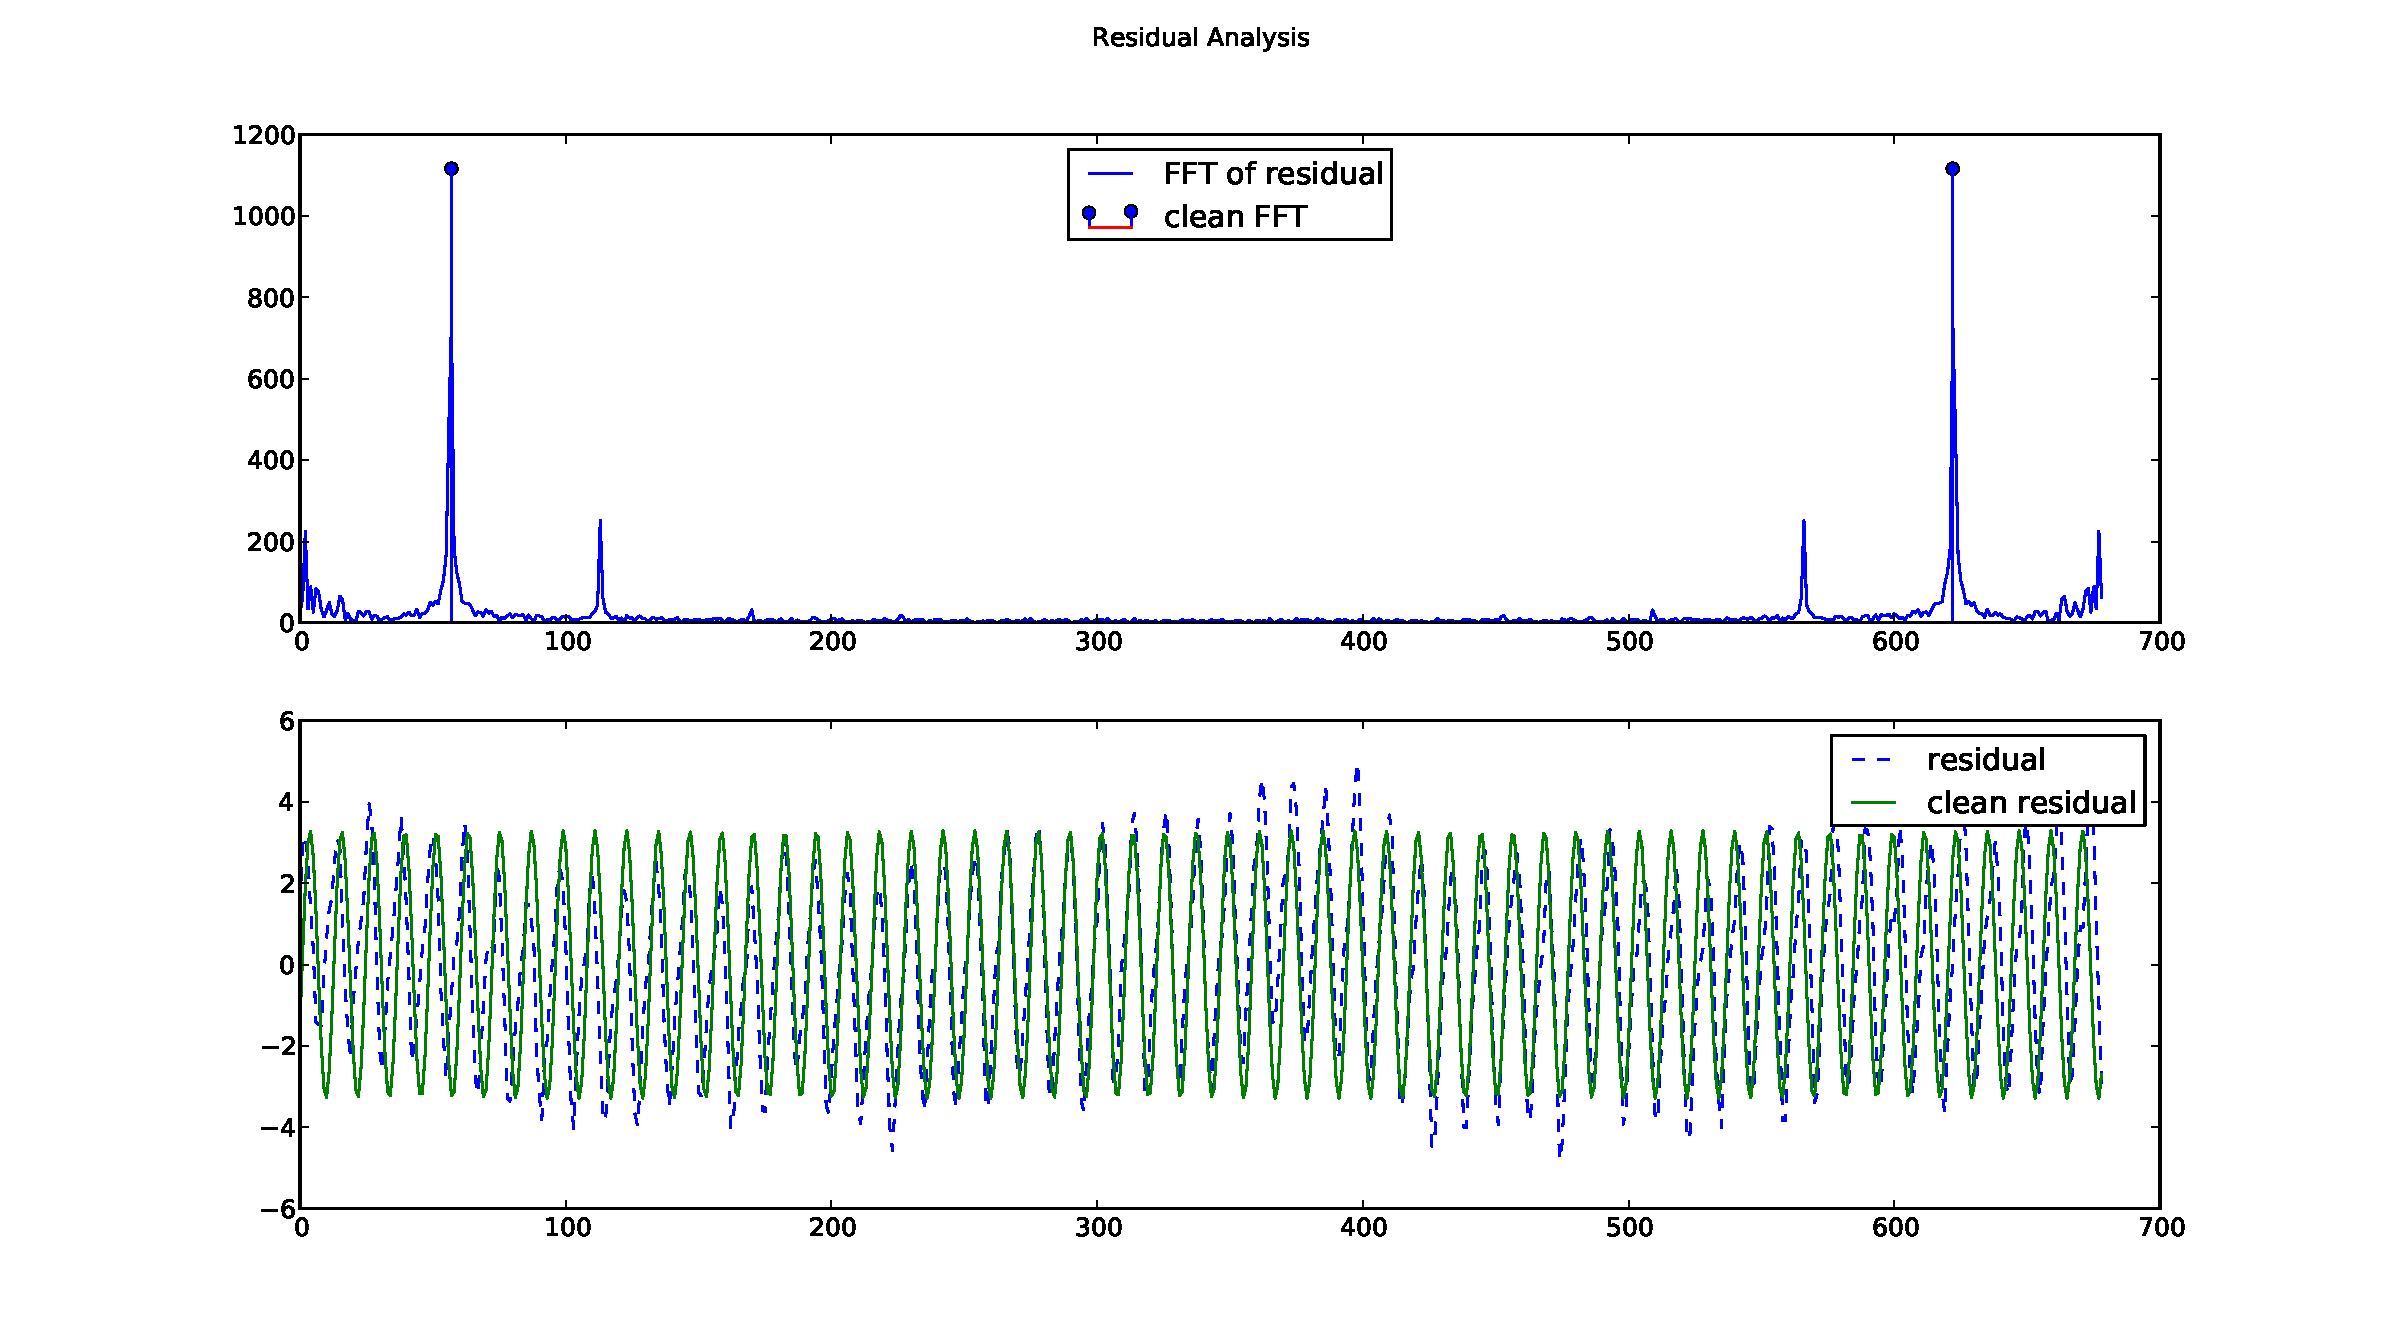
\includegraphics[width=18cm]{figs/co2_spectrum.pdf}
\caption[]{Spectrum of the residual (short-term trend) = $f_{CO_2}(t) - f_L(t)$.}
\label{fig:co2_spectrum}
\end{subfigure}\\
\begin{subfigure}[h]{\linewidth}
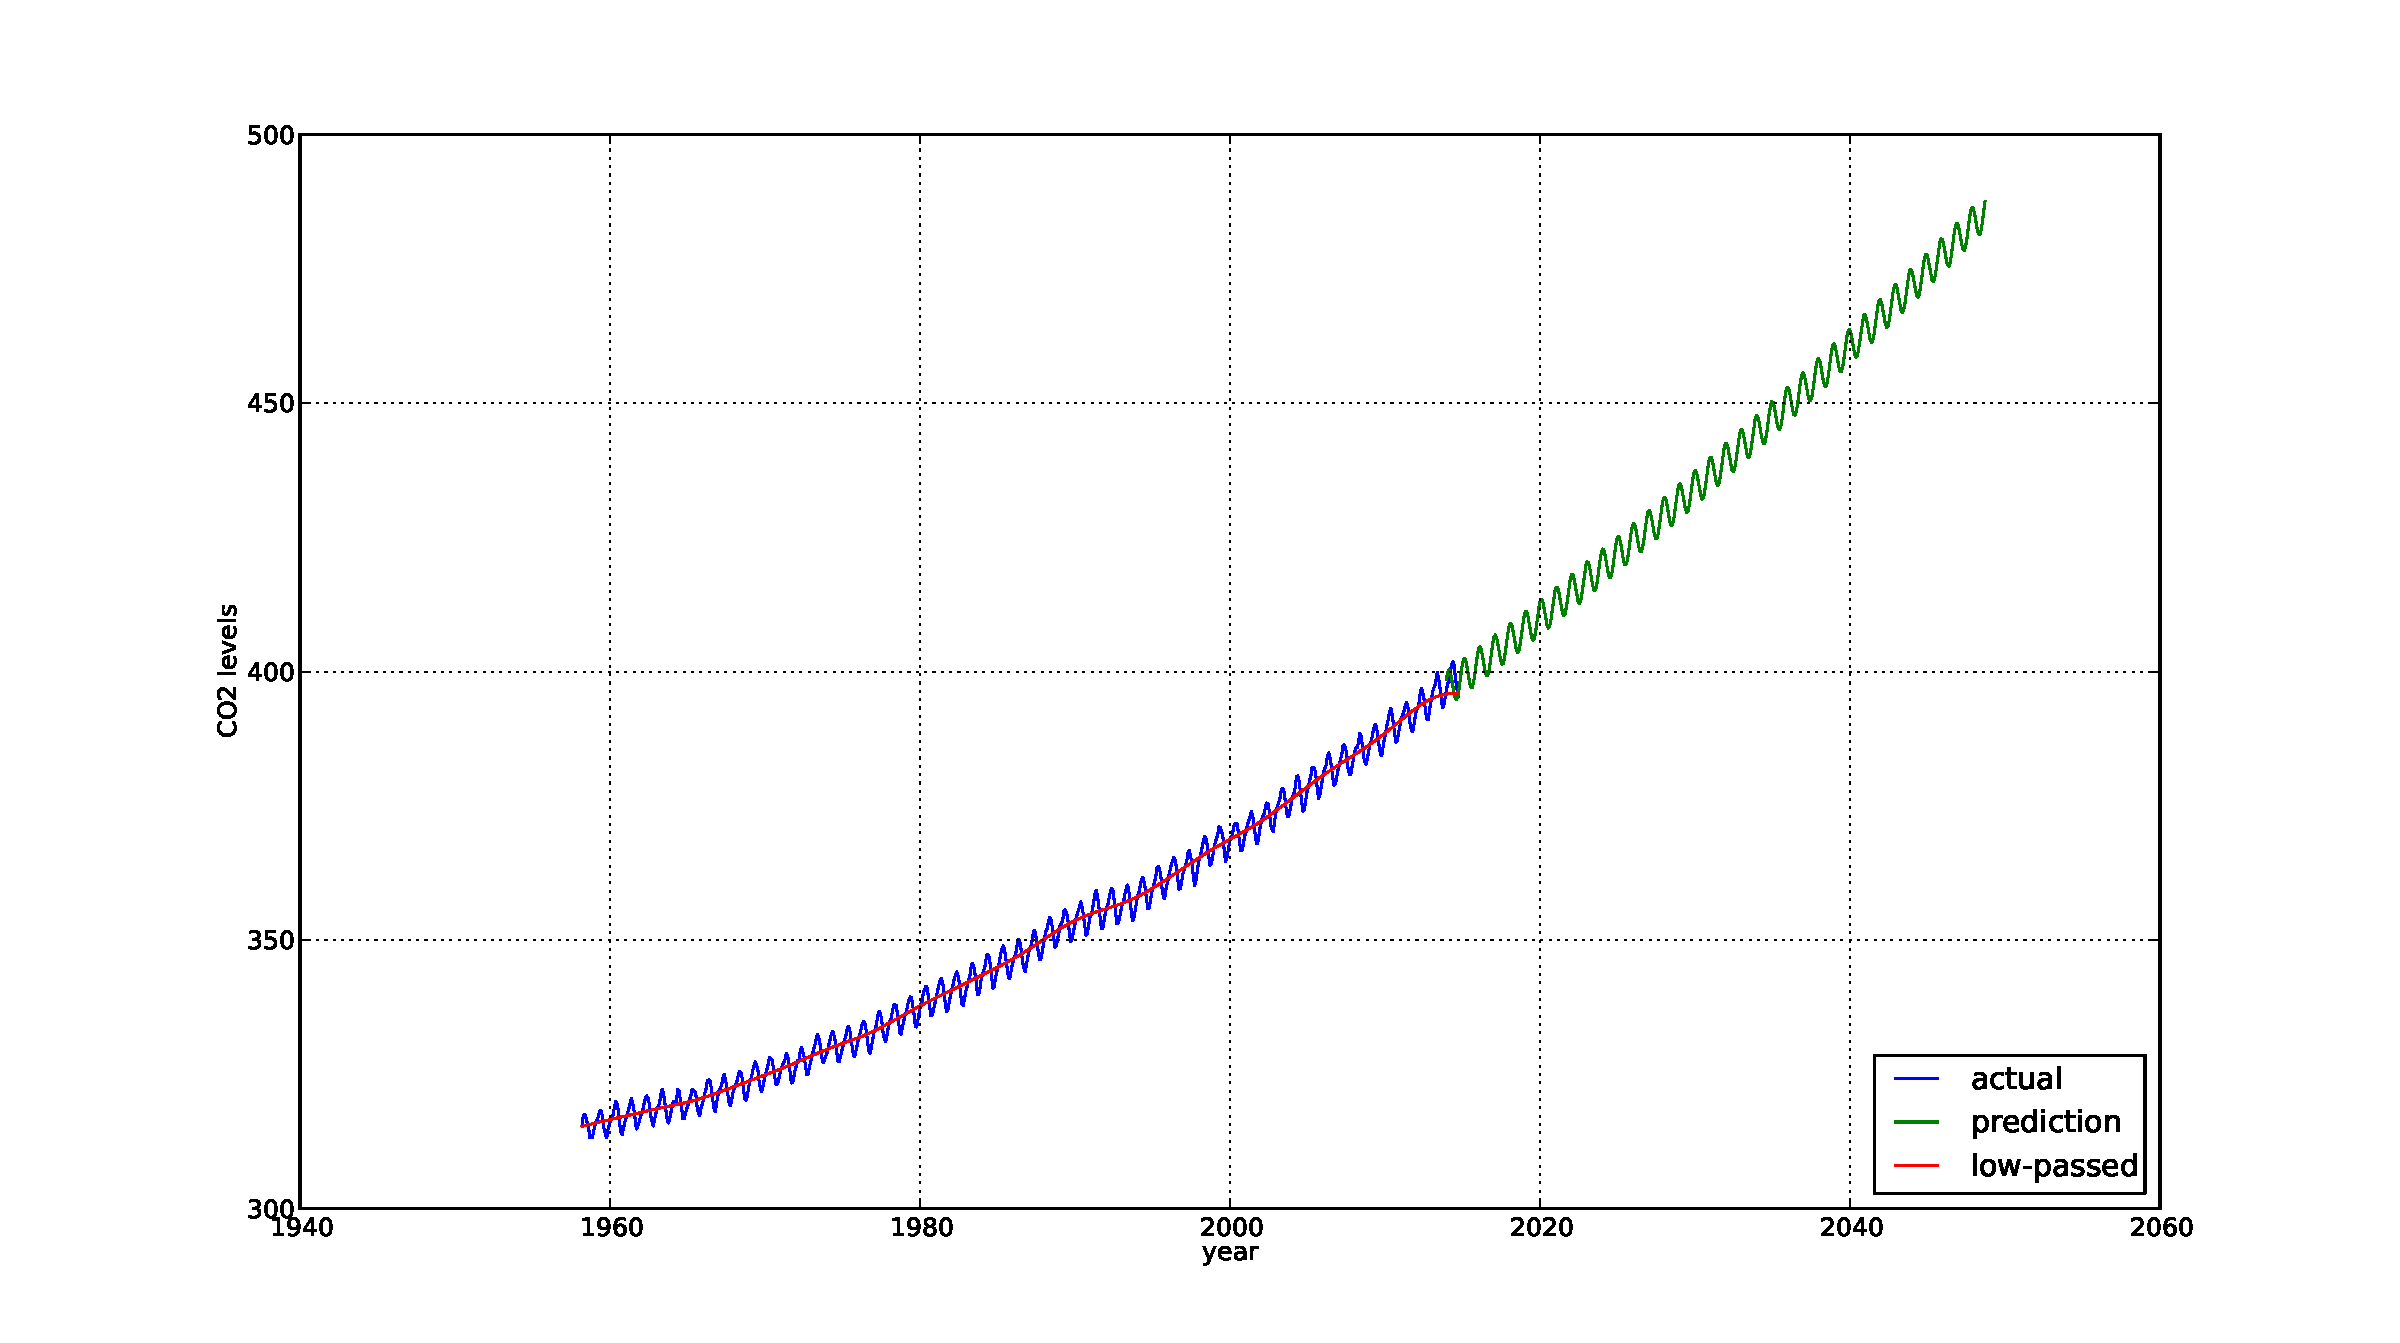
\includegraphics[width=18cm]{figs/co2_predict.pdf}
\caption[]{Prediction of $\text{CO}_2$ time series data.}
\label{fig:co2_decomp}
\end{subfigure}
\end{center}
\end{figure}

Figure~\ref{fig:co2_decomp} shows the final result --- predictions up to the year 2050. Also shown is the low-passed version of the original signal used for fitting the long-term trend.
\clearpage
\subsection*{Gaussian Process Regression for $\text{CO}_2$}
The code written for the \emph{Data Estimation and Inference}  course was used here. The polynomial fit for the long-term trend was used as the mean-function. For the covariance, I analysed two Kernels --- (1) Square-Exponential $= \sigma^2 exp\left(-(x_1-x_2)^2/2a\right) + \sigma_y^2I$ and, (2) Periodic $= \sigma^2 exp\left(-l^2\sin^2(2\pi/b|x_1-x_2|)\right)$. The hyper-parameters were optimised using a combination of conjugate gradient methods and human-in-the-loop-stochastic-gradient-descent.\\\\
Figure~\ref{fig:gpr} shows the results (please see the figure caption for discussion). 

\begin{figure}[htp]
\begin{center}
\begin{subfigure}[h]{\linewidth}
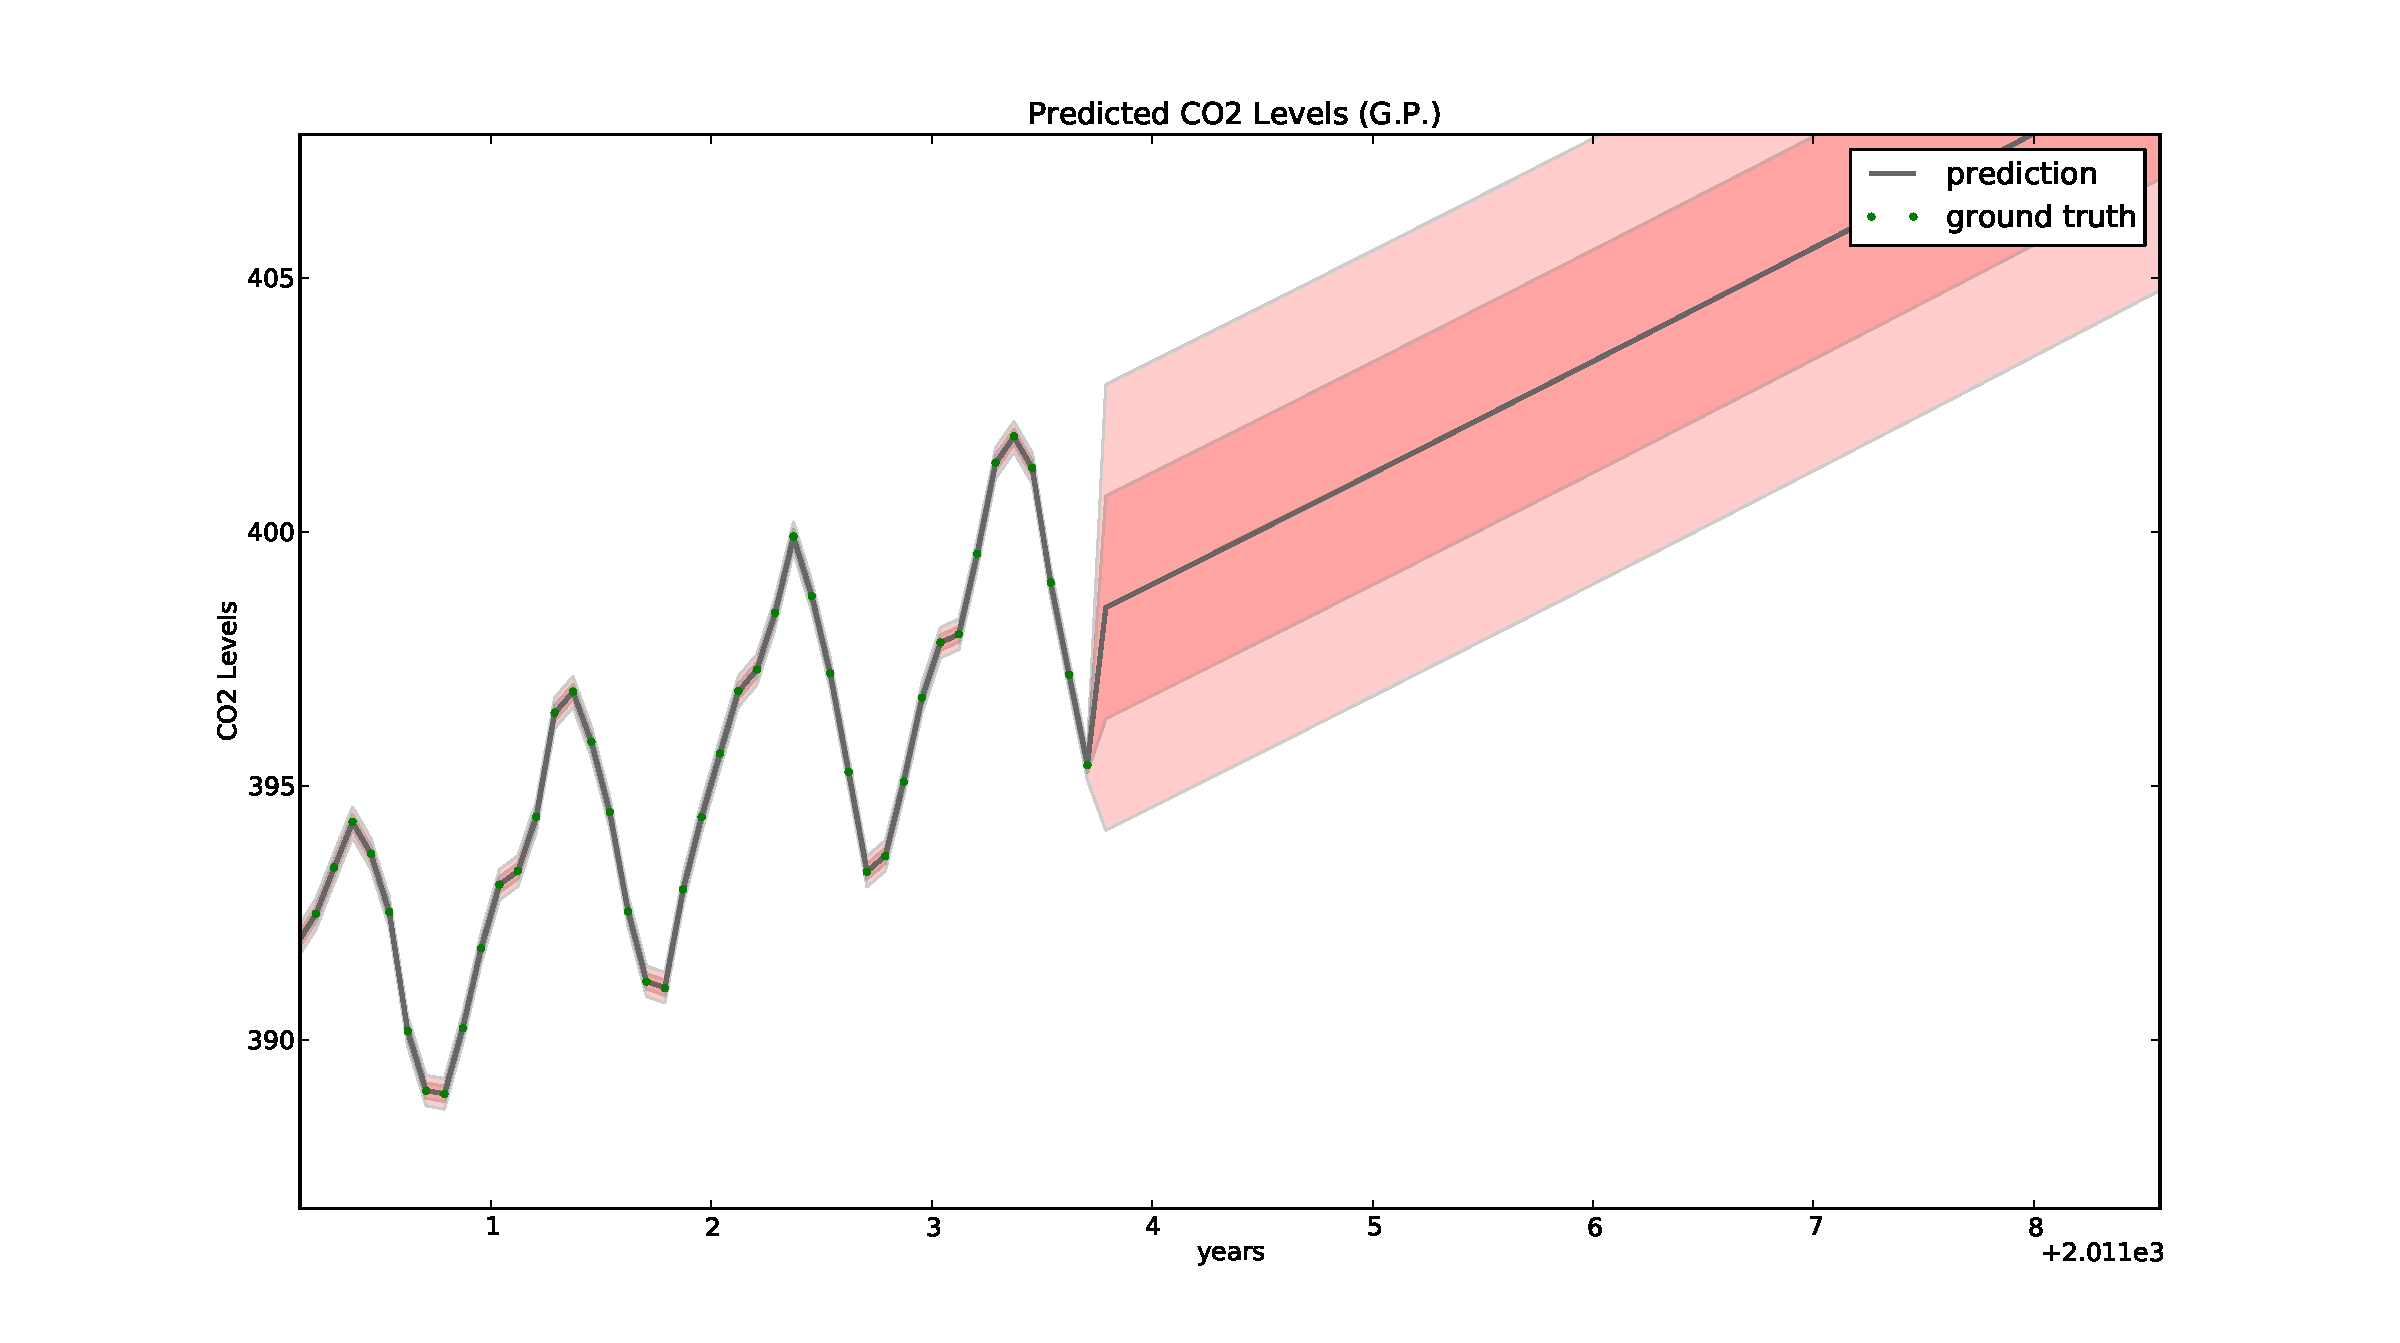
\includegraphics[width=18cm,height=6.5cm]{figs/co2_predict_gp.pdf}
\end{subfigure}\\
\begin{subfigure}[h]{\linewidth}
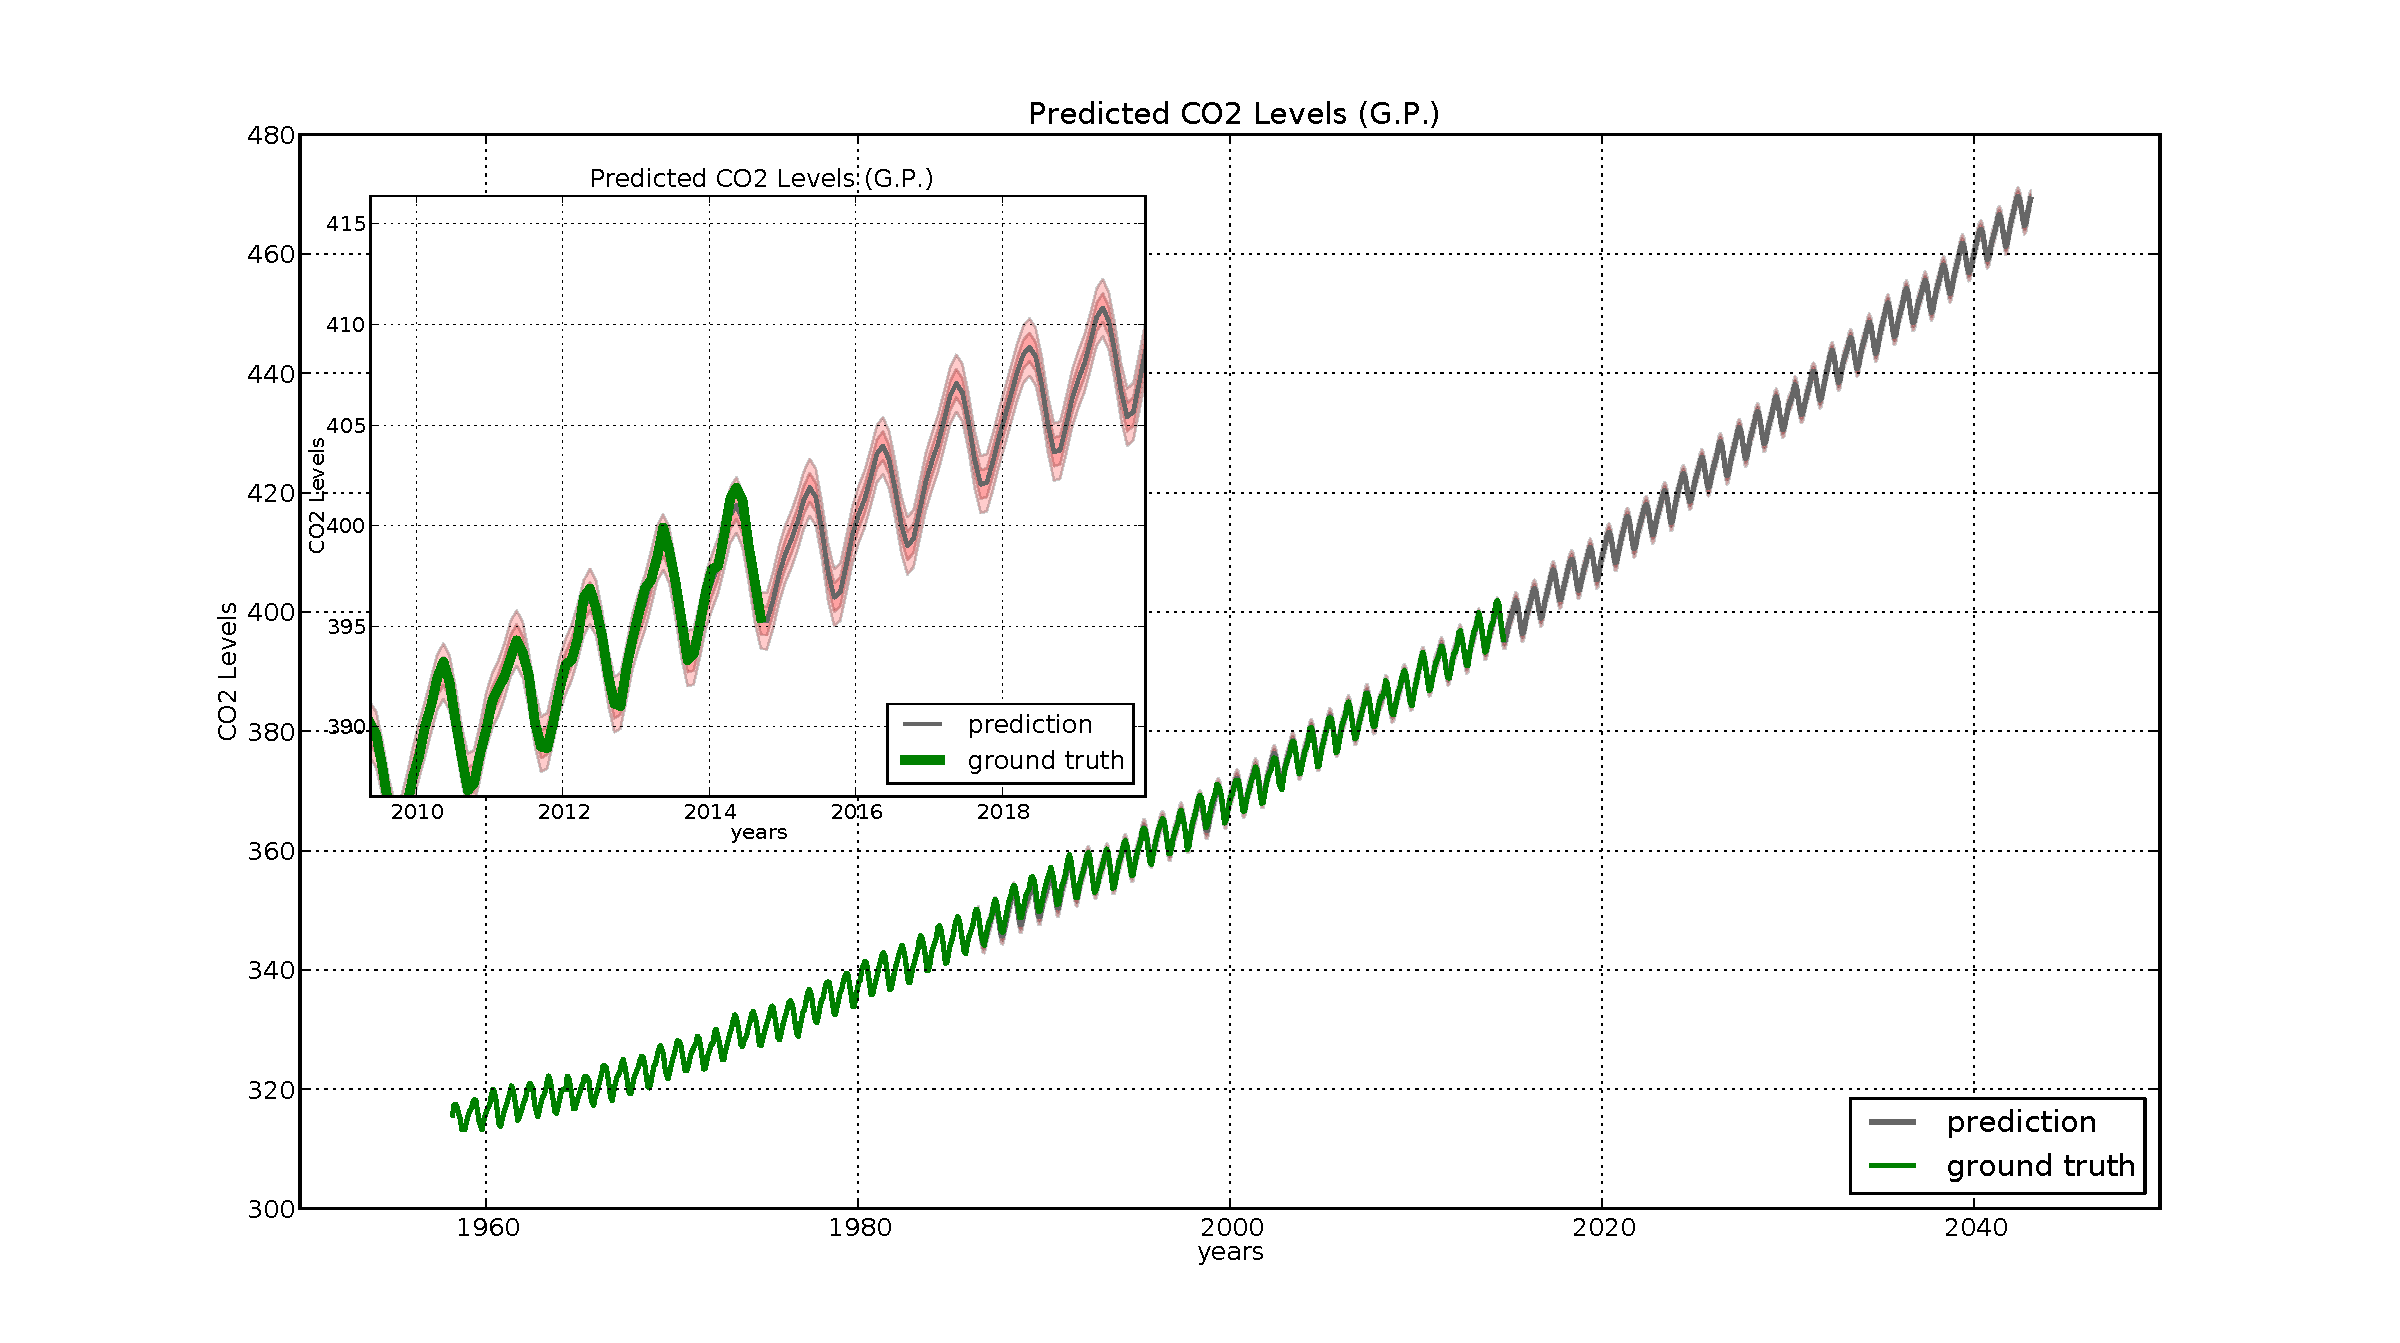
\includegraphics[width=18cm,height=6.5cm]{figs/co2_predict_gp_comb.pdf}
\end{subfigure}
\end{center}
\caption[]{[Top] GPR using the square-exponential kernel. Note the high-uncertainty in prediction. The future predictions basically just track the mean function. [Bottom] GPR prediction using periodic kernel. Since this periodic kernel captures the periodicity in the data, the future predictions have low uncertainty (inset). There is some finite variance at the points where observations are available because an observation uncertainty term was added to the kernel to make it numerically robust. The two red intervals indicate regions of one and two standard deviations.}
\label{fig:gpr}
\end{figure}
\clearpage

\section*{Sunspots Activity Forecasting}
This Sunspots Activity series was forecasted using two techniques --- (1) Using $AR(p)$ models trained using Yule-Walker equations and, (2) using 1-hidden layer feed-forward neural network regression with $p$ lagged inputs, trained using back-propagation.\\

A neural-network was used, because auto-regressive modes can be seen as a one linear neuron (perceptron) network. Hence, I was curious whether adding further complexity to the model improves the prediction accuracy. The neural network architecture was heuristically \footnote{keeping in mind the size of training data available and the time required to train these networks.} chosen to have one-hidden layer, with $p$ $tanh$ input units, $p/2$ $tanh$ hidden units and one linear output unit. The inputs to the network were $p$ delayed values of the signal $\{x[t-p],\hdots,x[t-1]\}$ and the output was trained to match $x[t]$. The data was normalised to have a mean of zero and a maximum value of one to avoid network saturation.\\

Both the AR model and the neural-network were trained for one-step predictions. However, 12 sequential  predictions (corresponding to one full year) were made using rolling regression in calculating the error rate. Figure~\ref{fig:ss} below shows the prediction output of $AR(15)$ model.
\begin{figure}[hbp]
\begin{center}
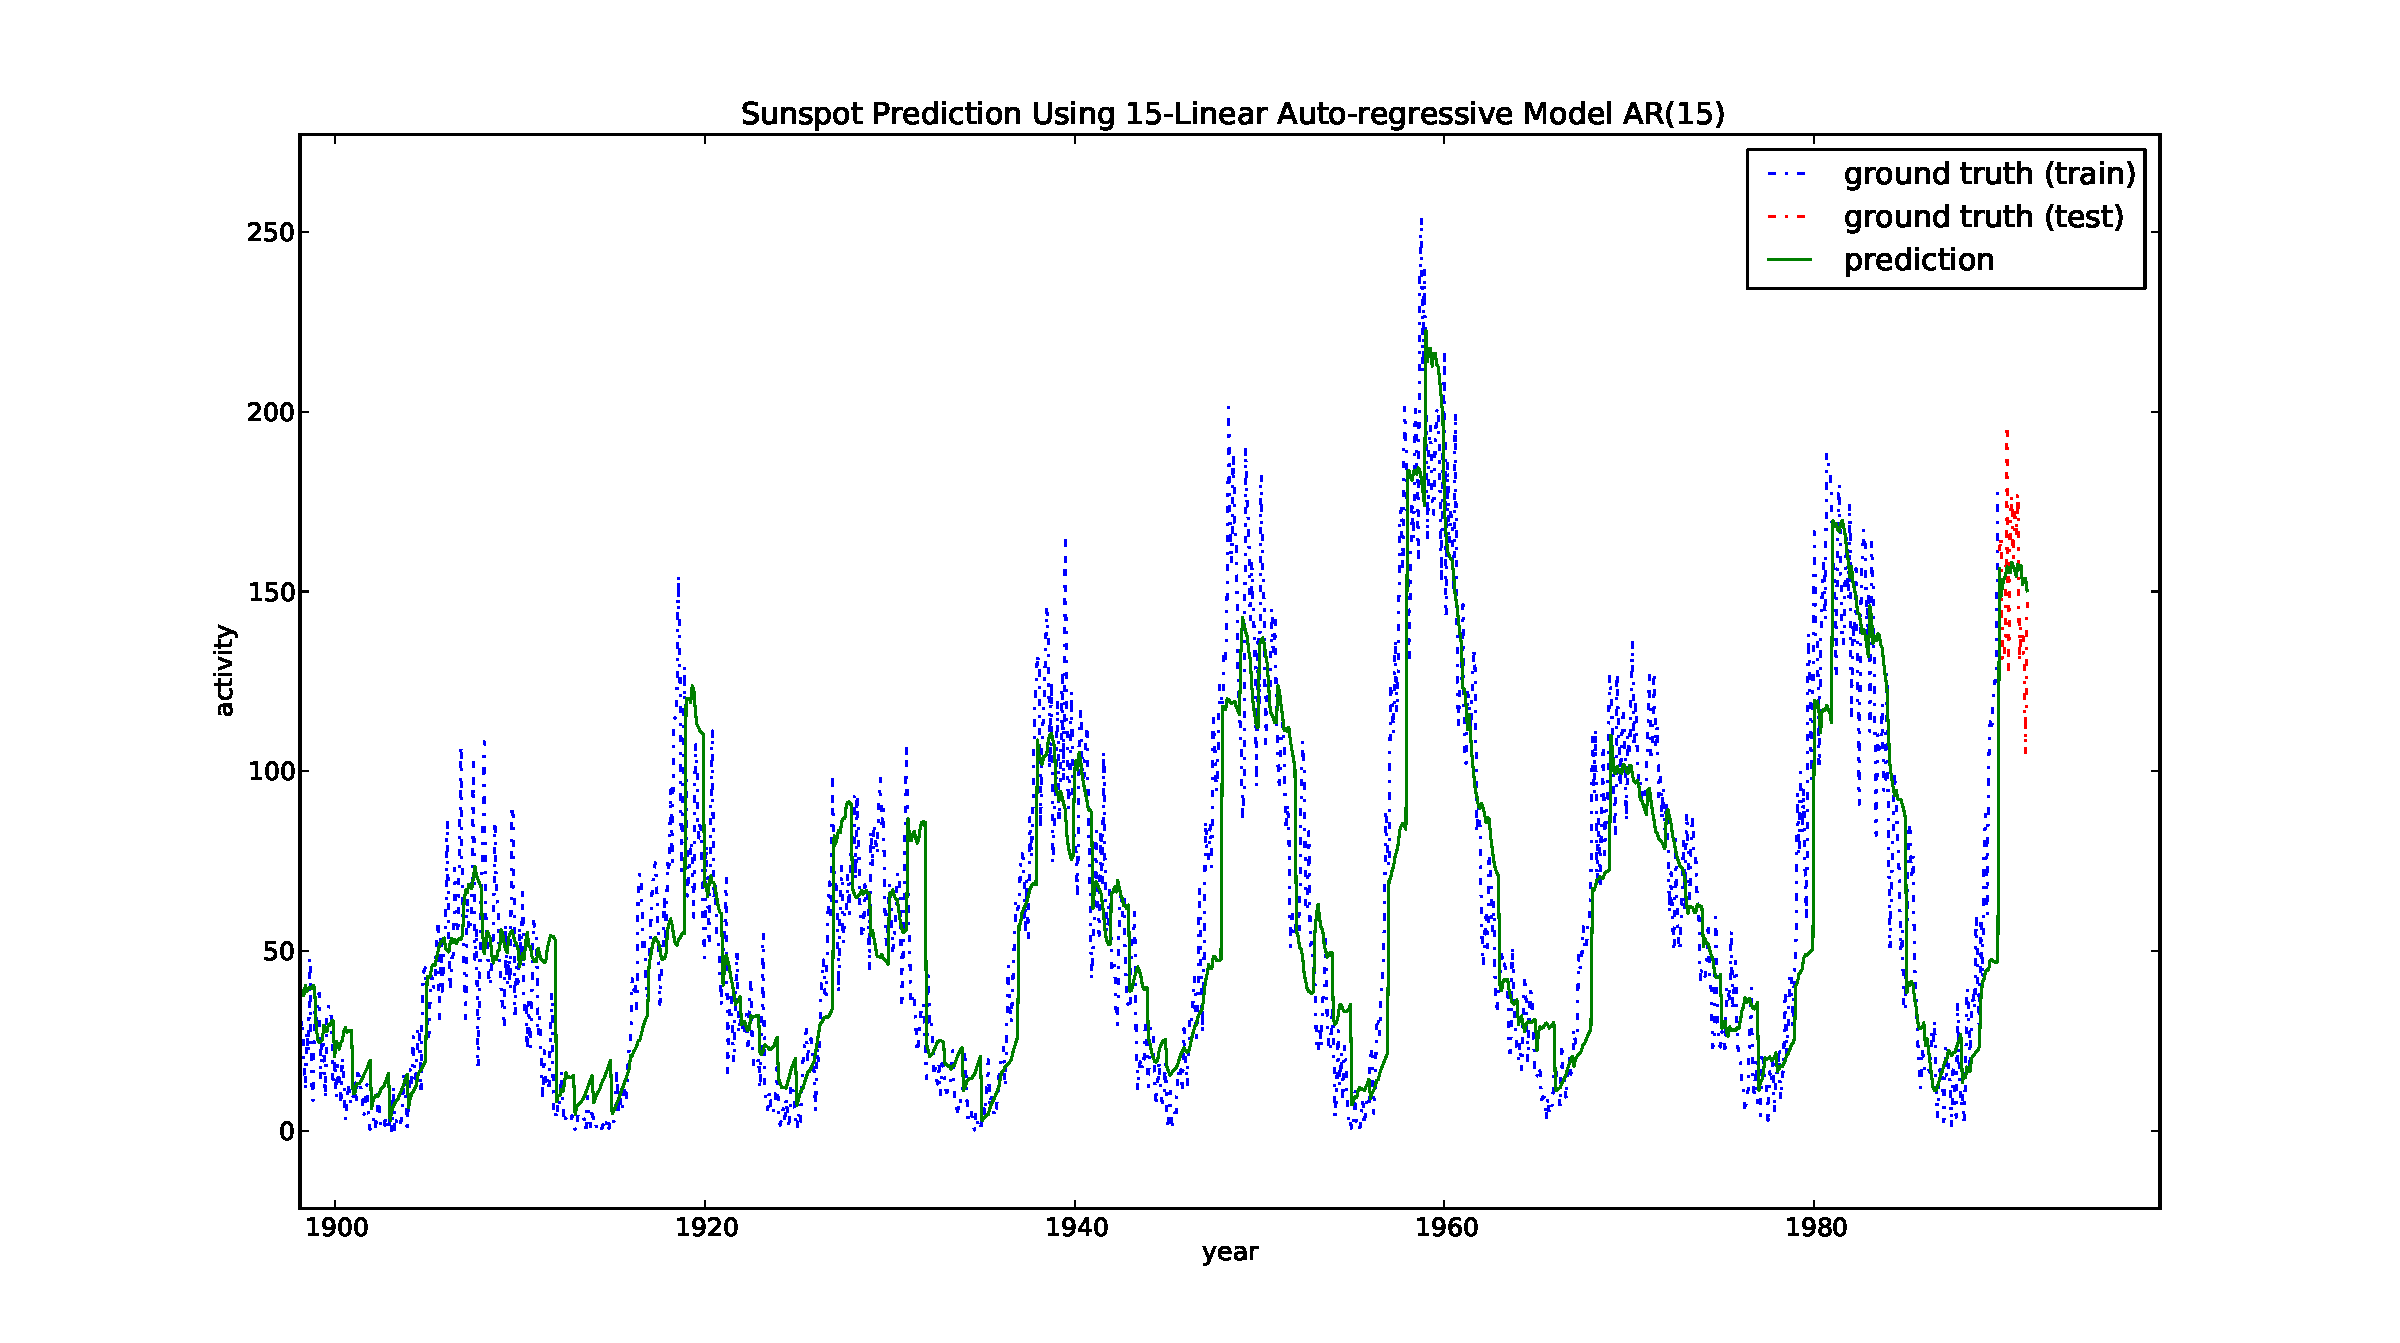
\includegraphics[width=18cm,height=9.5cm]{figs/ss_AR15_predict.pdf}
\end{center}
\caption[]{Sunspot data prediction using Auto-Regressive ($p=15$) model.}
\label{fig:ss}
\end{figure}
\clearpage

Figure~\ref{fig:ss_err} and compares the accuracy of the AR model and neural-network for increasing values of $p$. We note that for small $p$ neural network tracks the error rate of the AR models but tends to overfit and do worse for larger $p  > 100$.
\begin{figure}[htp]
\begin{center}
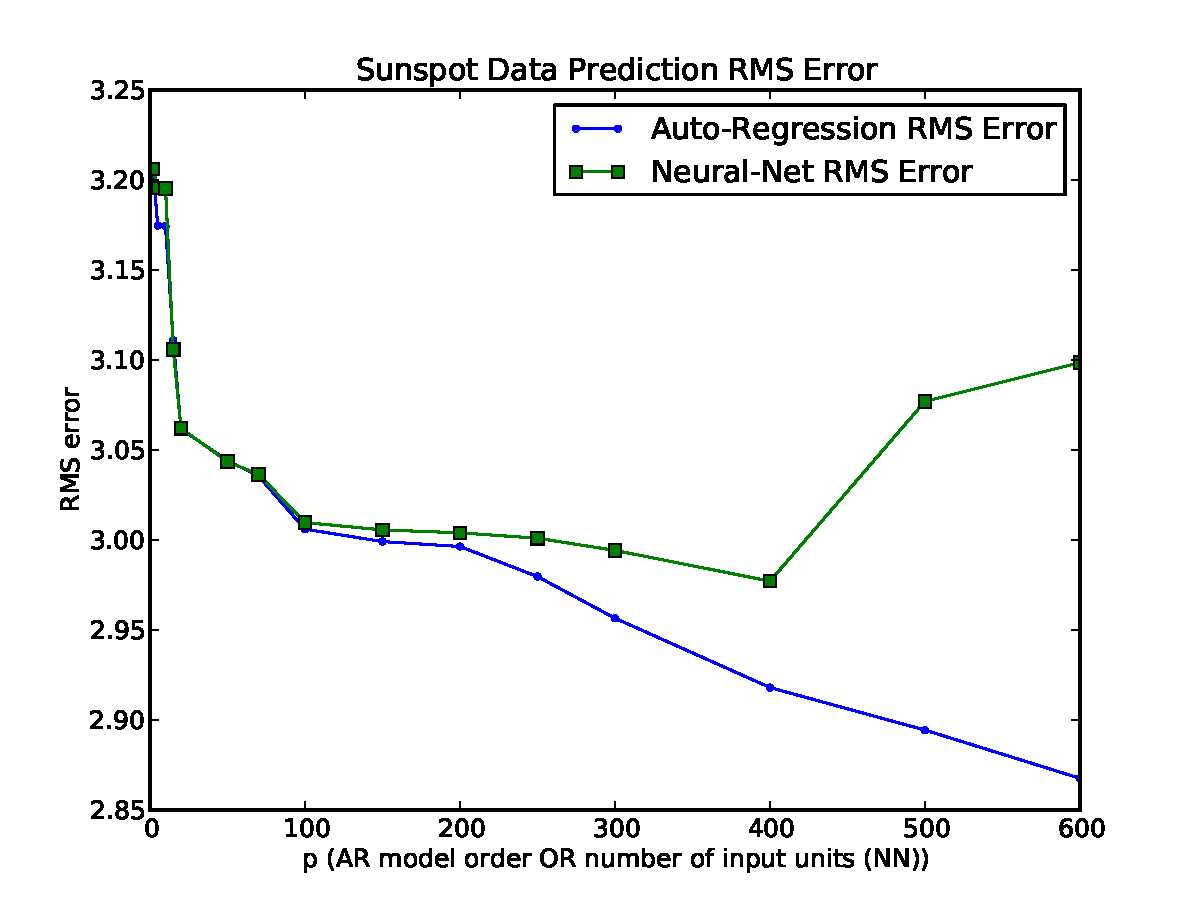
\includegraphics[width=10cm,height=6.5cm]{figs/sunspot_fit_error.pdf}
\end{center}
\caption[]{Sunspot data prediction using Auto-Regressive ($p=15$) model.}
\label{fig:ss_err}
\end{figure}

Both AR models and NN (for regression) invariably introduce some ``lag'', i.e., more concretely, the predictions of these models is better matched if is shifted in time by some small amount. To quantify this shift, I found the peak of the correlation function between the predicted signal and the actual signal. Figure~\ref{fig:ss_corr} shows the correlation function and peak for AR(15) model. Table~\ref{tab1} shows the amount of shift for optimum matching as a function of $p$ for AR models.
\begin{figure}[hbp]
\begin{center}
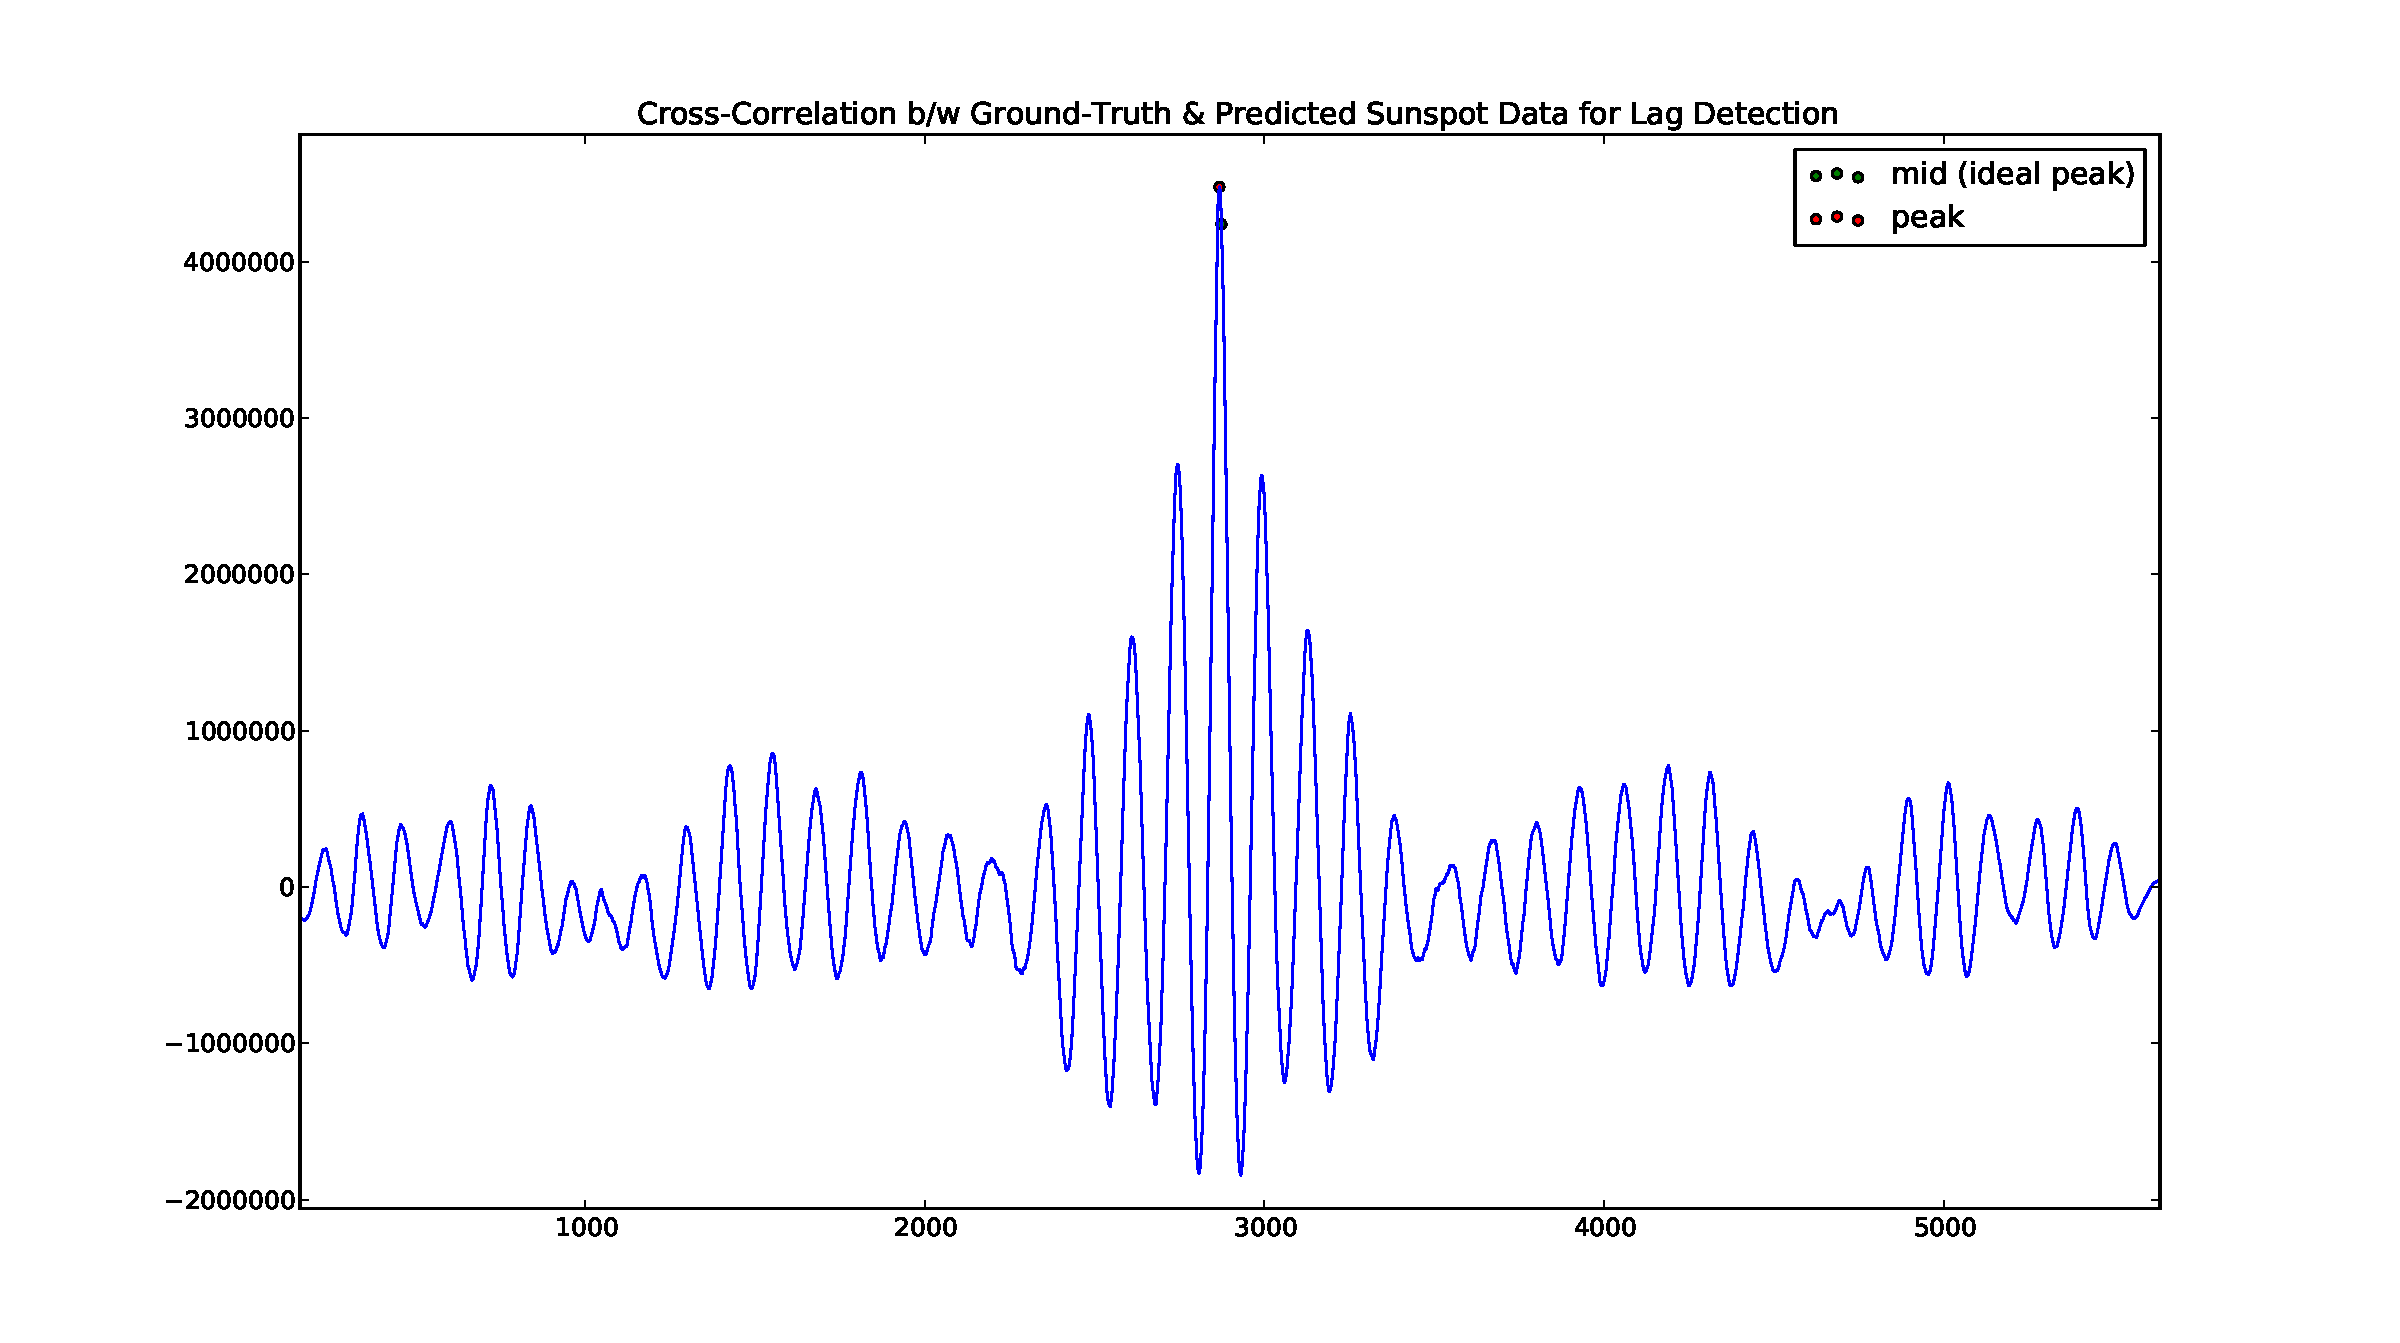
\includegraphics[width=18cm,height=6.5cm]{figs/ss_lag_corr.pdf}
\end{center}
\caption[]{Correlation between prediction and the actual signal for detecting lag.}
\label{fig:ss_corr}
\end{figure}

\begin{table}[htp]
\begin{center}
\begin{tabular}{|l||r|r|r|r|r|r|r|r|r|r|r|}
\hline
p      & 2 & 5 & 10 & 15 & 20 & 70 & 100 & 300 & 500 & 600\\\hline
Lag  & -5 &  -6 & -6 & -6 & -5 & -4 & -4 & -3 & 0 & 0 \\\hline
\end{tabular}
\caption{Lag for best correlation (or matching) as a function of $p$.}
\label{tab1}
\end{center}
\end{table}

\section*{Financial Data}
A distinctive feature of this data-set is that it is discrete\footnote{Thanks to James Thewlis and the TAs for this insight.} --- the financial data goes up or down in discrete units. Hence, predicting this time series can be seen as a classification problem instead of a regression problem --- given the past data, predict whether the change in the next tick will be $\{-4,\hdots,0,\hdots,4\}$.\\

All classification problems rely on find good features for their solution. Given the time constraints and my past (good) experience with using them for MNIST digit classification, I once again tried using neural networks\footnote{neural-networks = classification sledge-hammers?}, but with little success. I tried a bunch of different architectures but none could do better than random guessing --- i.e. an error rate better than $1/|\{-4,\hdots,0,\hdots,4\}| = 1/9$. Figure~\ref{fig:nn} shows the error-rate from a typical run --- we note that the neural network overfits to the training data and generalises poorly to the test-data. Perhaps, techniques to avoid overfitting would have helped here.

\begin{figure}[hbp]
\begin{center}
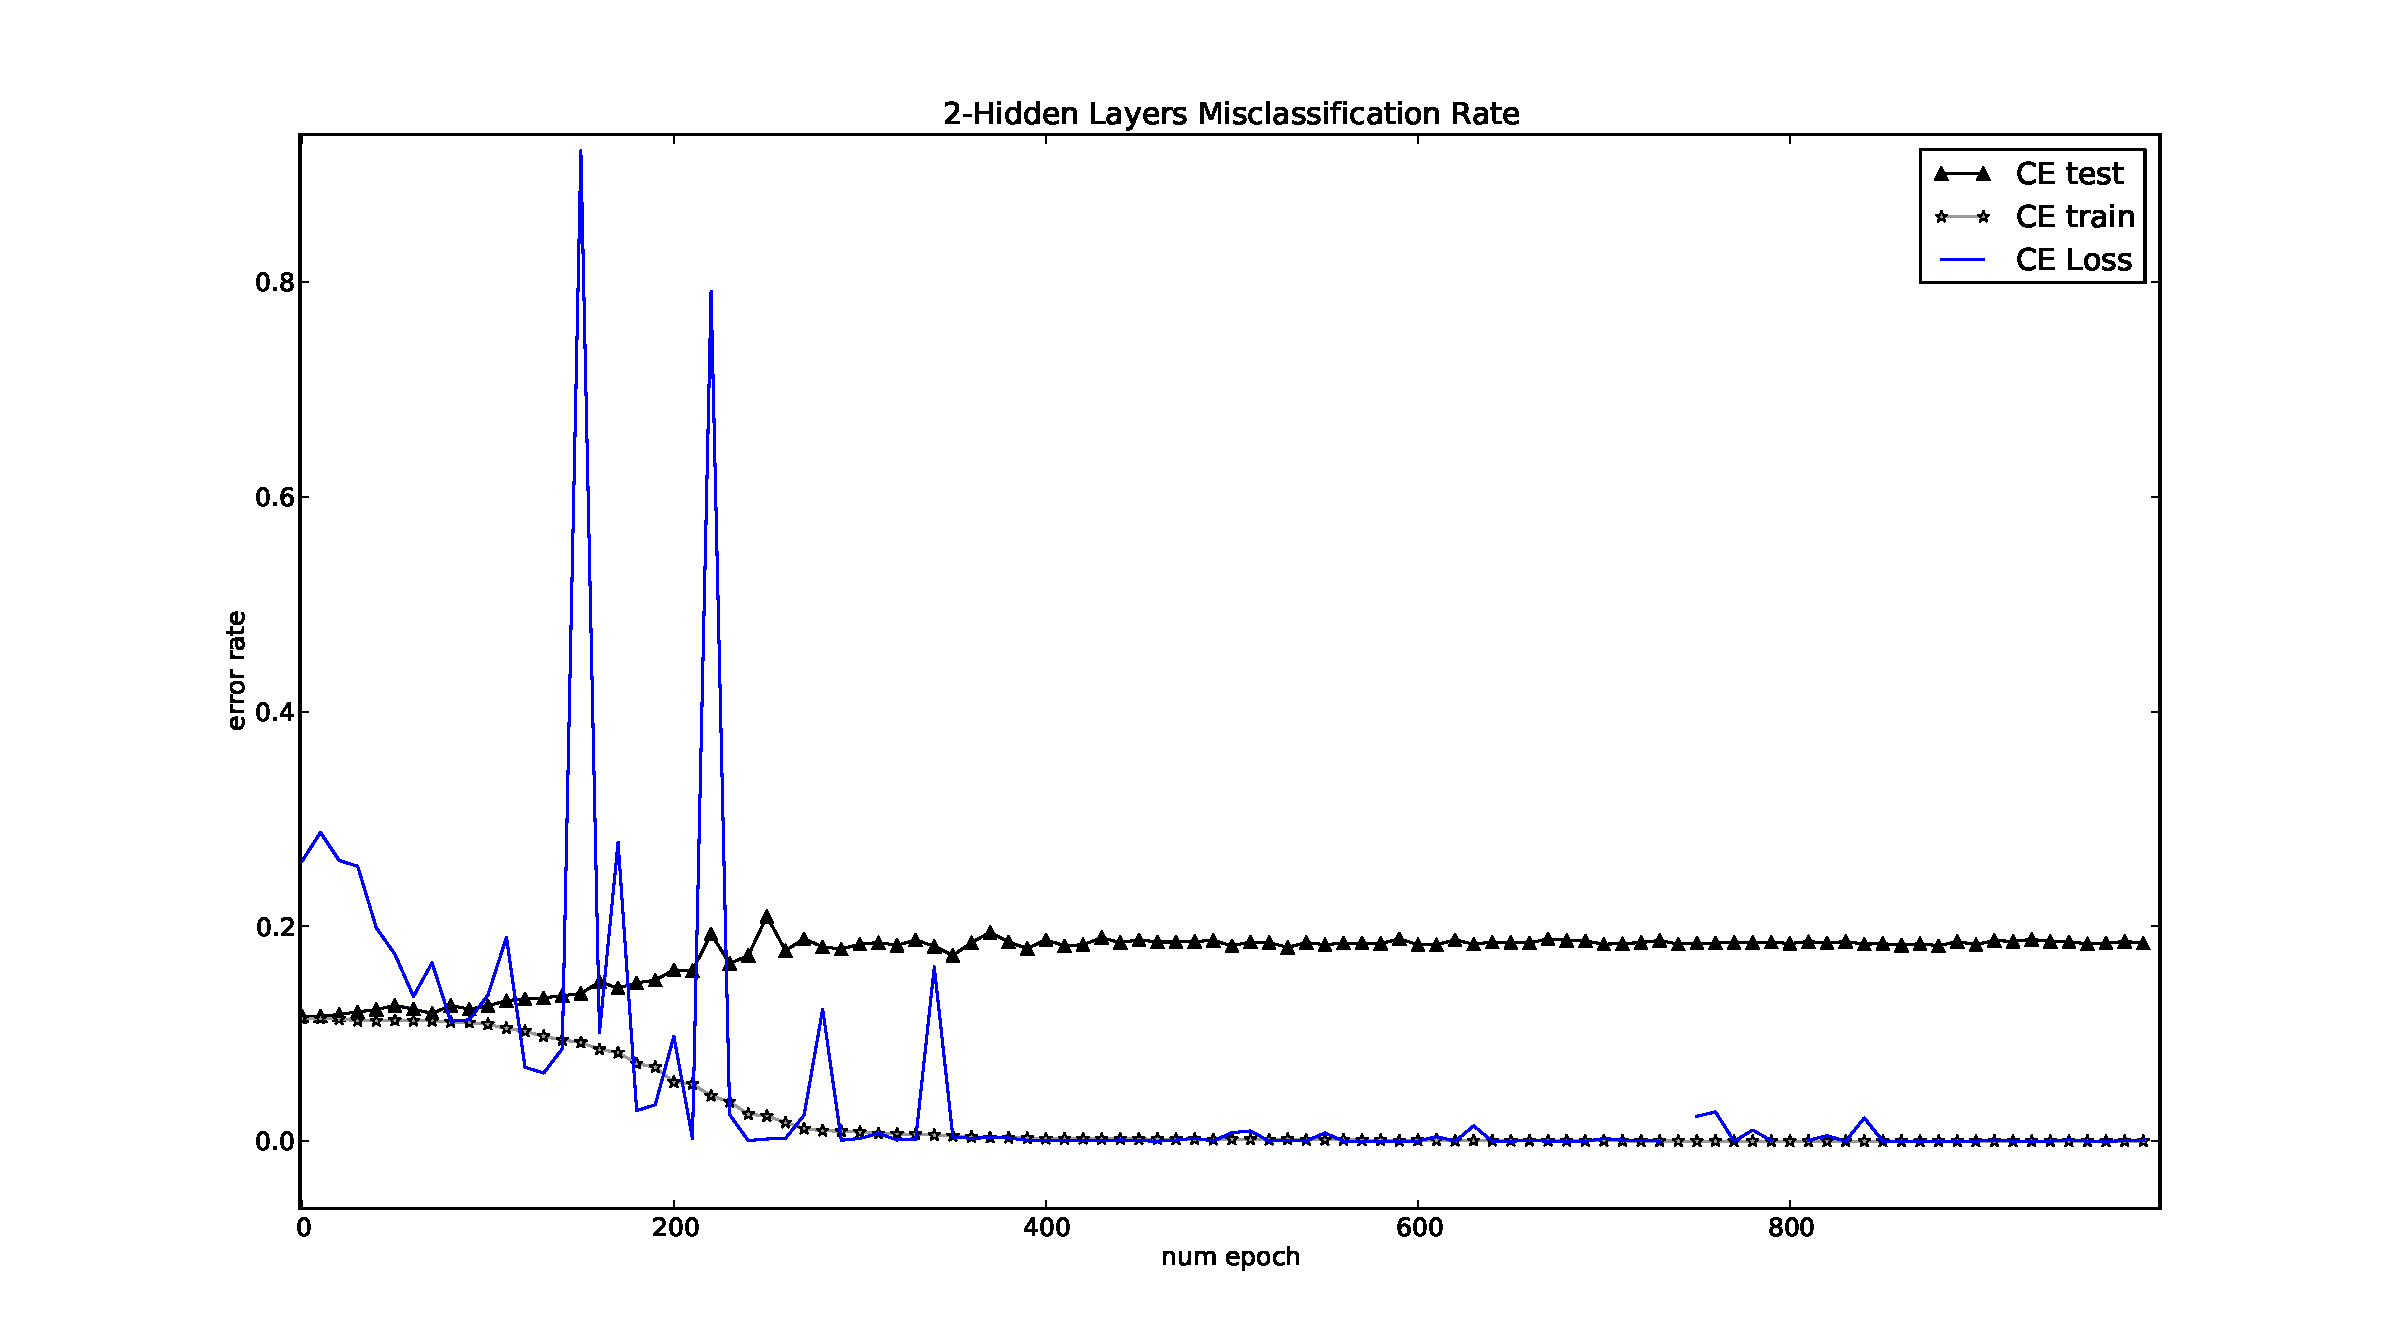
\includegraphics[width=18cm,height=8cm]{figs/two_layer_finance.pdf}
\end{center}
\caption[]{Cross-Entropy loss function error rate for a feed-forward neural network on the financial time series data.}
\label{fig:nn}
\end{figure}
\clearpage

\section*{Mackey-Glass Time Series}
Unfortunately, I could not find to really delve into this time series due to time constraints. While reading about solving this problem I came across the ideas of recovering embedding dimension and attractors --- things I would love to explore further in the future.
\section*{Code}
All the code was written in python. No time-series-forecasting/ machine-learning libraries were used. All the predictors --- AR model, gaussian process regression, neural nets were written by me and the source code is attached with this report. Instructions on how to run the code are present in \texttt{README.txt}
\section*{Thank You!}
\end{document}
